\documentclass{article}

\usepackage[final,main]{neurips_2026}
% \usepackage[main]{neurips_2026}

\usepackage[utf8]{inputenc}
\usepackage{natbib}
\usepackage[T1]{fontenc}
\usepackage{hyperref}
\usepackage{url}
\usepackage{booktabs}
\usepackage{amsfonts}
\usepackage{amsmath}
\usepackage{nicefrac}
\usepackage{xcolor}
\usepackage{graphicx}
\usepackage{multirow}
\usepackage{subcaption}
\usepackage{placeins}
\graphicspath{{figures/}}

\title{GORGO: Online Tuning for Cross-Region Network-Aware LLM Serving}

\author{
  Alessio Ricci Toniolo \\
  Carnegie Mellon University \\
  \texttt{atoniolo@andrew.cmu.edu} \\
  \And
  Rome Thorstenson \\
  Yale University \\
  \texttt{rome.thorstenson@aya.yale.edu} \\
  \And
  Abinaya Dinesh \\
  UC Berkeley \\
  \texttt{adinesh@berkeley.edu} \\
}

\begin{document}

\maketitle

\begin{abstract}
Increasingly, LLM inference services proxy client requests to engine replicas distributed globally.
Load-balancing policies must jointly account for
factors including KV-cache locality, replica load, and variable network latency when
optimizing for metrics like latency and TTFT.
However, existing systems only evaluate a subset of these factors in their cost
model, leading to uneven concentrations of load and KV-cache across replicas. We
present GORGO, a proxy architecture that holistically factors network latency,
prefill cost, and queueing delay using tunable parameters. Since open-source chat
datasets such as LMSYS-Chat-1M and WildChat-4.8M lack long-context, high
prefix-reuse data, we release a synthetic dataset, ART-Chat-2.5M, from
long-context production metadata. On a tuning window from ART-Chat-2.5M,
evolutionary strategies guide the GORGO policy's parameters to directly optimize
p95 TTFT. During held-out evaluation windows, we fix the parameter values learned
from tuning and improve p95 TTFT by 8--15\% and p95 end-to-end (E2E) latency by
15--31\% over baseline load balancing policies simple session affinity and prefix-cache.
The code and ART-Chat-2.5M dataset can be found at \href{https://github.com/Arcadia-Research-Team/GORGO}{https://github.com/Arcadia-Research-Team/GORGO}.
\end{abstract}

% -----------------------------------------------------------------------
\section{Introduction}
\label{sec:intro}
% -----------------------------------------------------------------------

In LLM serving systems, perceived latency to the user is dominated by the time-to-first-token (TTFT). On a single replica, TTFT is dominated by three costs: (i) prefill time, (ii) round trip time (RTT) from client (proxy) to replica, and (iii) queueing delay behind in-flight requests. Prefix-caching, which is enabled in inference engines SGLang \citep{sglang2024} and vLLM \citep{vllm2023}, eliminates the prefill cost of previous turns in a multi-turn conversation. As LLM context windows increase in length, the time saved by prefix caching 90\% of a prompt with 100,000 tokens reduces the prefill cost to 10,000 tokens and decreases TTFT substantially.

Since LLM deployments proxy requests to inference engines across regions, the cost savings of prefix-caching depend on choosing a replica with the request session's prefix. Popular routing policies such as consistent hashing and prefix reuse aim to distribute load evenly while creating affinity between a session's requests and replica(s) to maximize KV-cache reuse \citep{karger1997consistent, chord2003, sglang2024, skywalker}. In compute-constrained regimes, bursty workloads can saturate a high-affinity replica, causing head-of-line (HOL) queueing delays from decode memory contention and negating cost savings from prefix-cache reuse. Routing policies that holistically evaluate all costs related to TTFT can maintain high prefix-cache reuse while minimizing the negative effects of load saturation and heterogeneous network latency.

Existing load balancing policies such as least-load, session affinity, and prefix-reuse may account for replica load or KV-cache hit rate; however, no existing policies consider network latency in cross-region scenarios, which can range on the order of 10ms to 1s (Figure~\ref{fig:rtt}). GORGO's routing policy accounts for all three TTFT costs, normalizes the units of measurement via tunable parameters, and jointly optimizes parameters through online tuning on real user workloads. To tune and stress-test different routing policies, in (\S\ref{sec:characterization}) we compile a LLM traffic trace from real production requests with high prefix-reuse and long-context prompts. The trace follows Mooncake's FAST'25 format \citep{qin2024mooncake} containing per-request timestamps, which can be linearly scaled to simulate variable saturation profiles.

We benchmark GORGO on a series of user workloads from ART-Chat-2.5M, our sensitized production Mooncake trace, and sweep across variable time scales to effectively saturate replicas without simulating unrealistic HOL queueing delay. Over existing load balancing policy baselines, GORGO jointly balances optimal TTFT with request concentration across replicas. Under the continuous batching paradigm, the ES-driven hillclimb tuner exploits warmer replicas close to the proxy and dramatically reduces TTFT at the cost of end-to-end (E2E) latency. We map the pareto frontier of request concentration across replicas, which explodes E2E latency for unbalanced distributions, and TTFT. Our contributions help contextualize the performance of LLM proxy routing policies in real-world user workloads, and (\S\ref{sec:results}) lists a case-by-case scenario of when one would want to use aforementioned baseline policies, the online GORGO policy, and offline GORGO with held-out weights. Finally, we show how conditioning the GORGO cost model on proxy-recorded replica load mitigates subversion of TTFT via continuous batching and slashes request latency across a panoply of metrics.

% -----------------------------------------------------------------------
\section{GORGO}
\label{sec:method}
% -----------------------------------------------------------------------

\subsection{Cost Model}

TTFT is known to consist of three different costs: network latency, prefill time, and queueing delay \citep{banaserve2025}. The KV-Cache, which stores key-value pairs of input sequences, removes redundant prefill computation for user sequences sharing a prefix with previously computed sequences \citep{sglang2024}. In a cross-region deployment setting, for an inference engine replica $i$ holding a set of cached token prefixes $c_i$, the cost of TTFT can be defined as the following function, where $x_r$ is the input sequence of tokens for a request $r$ and the prefill time depends only on the set difference $(x_r \setminus c_i)$, the tokens in $x_r$ not already cached on $i$:

\begin{equation}
\mathrm{TTFT} = T_{\texttt{network}}(i) + T_{\texttt{queue}}(i) + T_{\texttt{prefill}}(x_r \setminus c_i)
\label{eq:ttft}
\end{equation}

Theoretically, $T_{\texttt{network}}$ and $T_{\texttt{queue}}$ correspond with round trip time from a client to server and the duration of request processing ahead of the incoming request $r$. However, inference engines support batching requests continuously in order to minimize waiting for completion of previous request processing \citep{orca2022}. While continuous batching allows admission of a new request into the currently running batch, the batch size is still bounded by a maximum number of concurrent requests and the available KV-cache budget, a critical knob that governs how much load a replica can admit before further requests wait in a queue \citep{vllm2023}.

In a distributed system, the temporal delay of retrieving queueing metrics from an engine replica makes cost evaluation challenging. We represent the input to $T_{\texttt{queue}}$ as the total number of tokens of requests without a completion event on the client proxy. $T_{\texttt{network}}$ is measured trivially as the exponential weighted moving average of a ping's round trip time from client proxy to server.
\begin{equation}
\mathrm{TTFT} = T_{\texttt{network}}(\mathrm{RTT}_i) + T_{\texttt{queue}}\left(i, \sum_{j=1}^{n_r} x_j\right) + T_{\texttt{prefill}}(x_r \setminus c_i)
\label{eq:ttft-proxy}
\end{equation}

\bigskip
\subsection{GORGO Proxy Design}

The GORGO proxy routes client requests to the engine replica with the minimum calculated cost from Equation~\ref{eq:ttft-proxy}, parameterized by weights $W_{\texttt{rtt}}$, $W_{\texttt{prefill}}$, and $W_{\texttt{queue}}$. These parameters weight the inputs $T_{\texttt{network}}$, $T_{\texttt{queue}}$, and $T_{\texttt{prefill}}$, which unfairly mixes the units of time and tokens, to normalize the correlated costs of latency, prefill cost, and queueing time on TTFT. The weight of $T_{\texttt{prefill}}$ is fixed to 1 because GORGO proxy makes routing decisions based on relative replica cost: only the ratio of weights matters in this design.
\begin{equation}
\mathrm{TTFT} = W_{\texttt{rtt}} * T_{\texttt{network}}(\mathrm{RTT}_i) + W_{\texttt{queue}} * T_{\texttt{queue}}\left(i, \sum_{j=1}^{n_r} x_j\right) + T_{\texttt{prefill}}(x_r \setminus c_i)
\label{eq:score}
\end{equation}

GORGO proxy uses a simple (1+1) evolutionary strategy to tune weights $W_{\texttt{rtt}}$ and $W_{\texttt{queue}}$ on the objective function, P95 TTFT.
Each parent weight $x_{t,k}$ is perturbed multiplicatively in log-space by a normal random variable $z_k$ times step size $\sigma$, and the new offspring weight $x_k'$ is clamped to values in the hyperparameter range $[lo_k, hi_k]$ where $lo_k > 0$ and $hi_k > 0$.

\begin{equation}
x_k' = \mathrm{clip}\left(\exp(\ln(x_{t,k}) + \sigma_t * z_k), [lo_k, hi_k]\right)
\end{equation}

When $x'$ beats the parent weight $x_t$ on the objective metric, the incumbent weight $x_{t+1}$ is updated to $x'$, and $\sigma$ is adjusted to maintain Rechenburg's 1/5 success rate of 1 accepted offspring for every 5 offspring.

% -----------------------------------------------------------------------
\section{Dataset}
\label{sec:characterization}
% -----------------------------------------------------------------------

Existing LLM chatbot datasets lack two critical components for benchmarking
cache-aware policies: (i) prefill-bound requests with long-context prompts and
(ii) multi-turn workloads with high prefix-reuse between requests. For example,
we measure the average request length and global prefix reuse of
\textbf{LMSYS-Chat-1M}~\citep{lmsys2024} and \textbf{WildChat-4.8M}~\citep{wildchat2024},
two popular LLM datasets derived from public chatbot demos
(Table~\ref{tab:datasets}, Figure~\ref{fig:dataset_combined}). WildChat-4.8M
contains hashed IPs per request, allowing categorization of cross-user and
intra-user reuse while LMSYS-Chat-1M lacks user identification. Additional
results from benchmarking GORGO on WildChat-4.8M can be found in
Appendix~\ref{app:wildchat}. Cache-aware policies provide no measurable gains
over simple baseline policies like \texttt{random} when routing requests with a
length of $<$3{,}000 tokens.

\textbf{ART-Chat-2.5M} is a long-context, multi-turn dataset synthetically generated from
a week-long metadata trace of production inference traffic with the same
prefix-reuse structure as the original workload. We release a replay-ready trace
in the Mooncake FAST'25 format, which contains per-request timestamps, request
metadata, and synthetically generated chat completion data~\citep{qin2024mooncake}.
By storing request timestamps, one can linearly scale the time between requests
to control replica load. We characterize the dataset against WildChat-4.8M and
LMSYS-Chat-1M in Table~\ref{tab:datasets} and Figure~\ref{fig:dataset_combined}.
Notably, the intra-user prefix reuse and average token length in ART-Chat-2.5M
are 19$\times$ and 6$\times$ higher than in WildChat-4.8M.

\begin{table}[t]
\centering
\small
\caption{Dataset. ART-Chat-2.5M contains higher average input tokens and global prefix reuse, which is measured by
adding the intra-user reuse and cross-user reuse, over other chat datasets.
}
\label{tab:datasets}
\begin{tabular}{lrrrrr}
\toprule
Dataset & Total reqs & Users & Avg input tokens & Intra-user reuse & Global reuse \\
\midrule
LMSYS-Chat-1M & 1{,}000{,}000 & --- & 467 & --- & 3.4\% \\
WildChat-4.8M & 3{,}199{,}860 & 1{,}833{,}730 & 2{,}925 & 4.7\% & 32.5\% \\
ART-Chat-2.5M & 2{,}525{,}215 & 4{,}984 & 17{,}964 & 89.4\% & 89.7\% \\
\bottomrule
\end{tabular}
\end{table}

\begin{figure}[t]
\centering
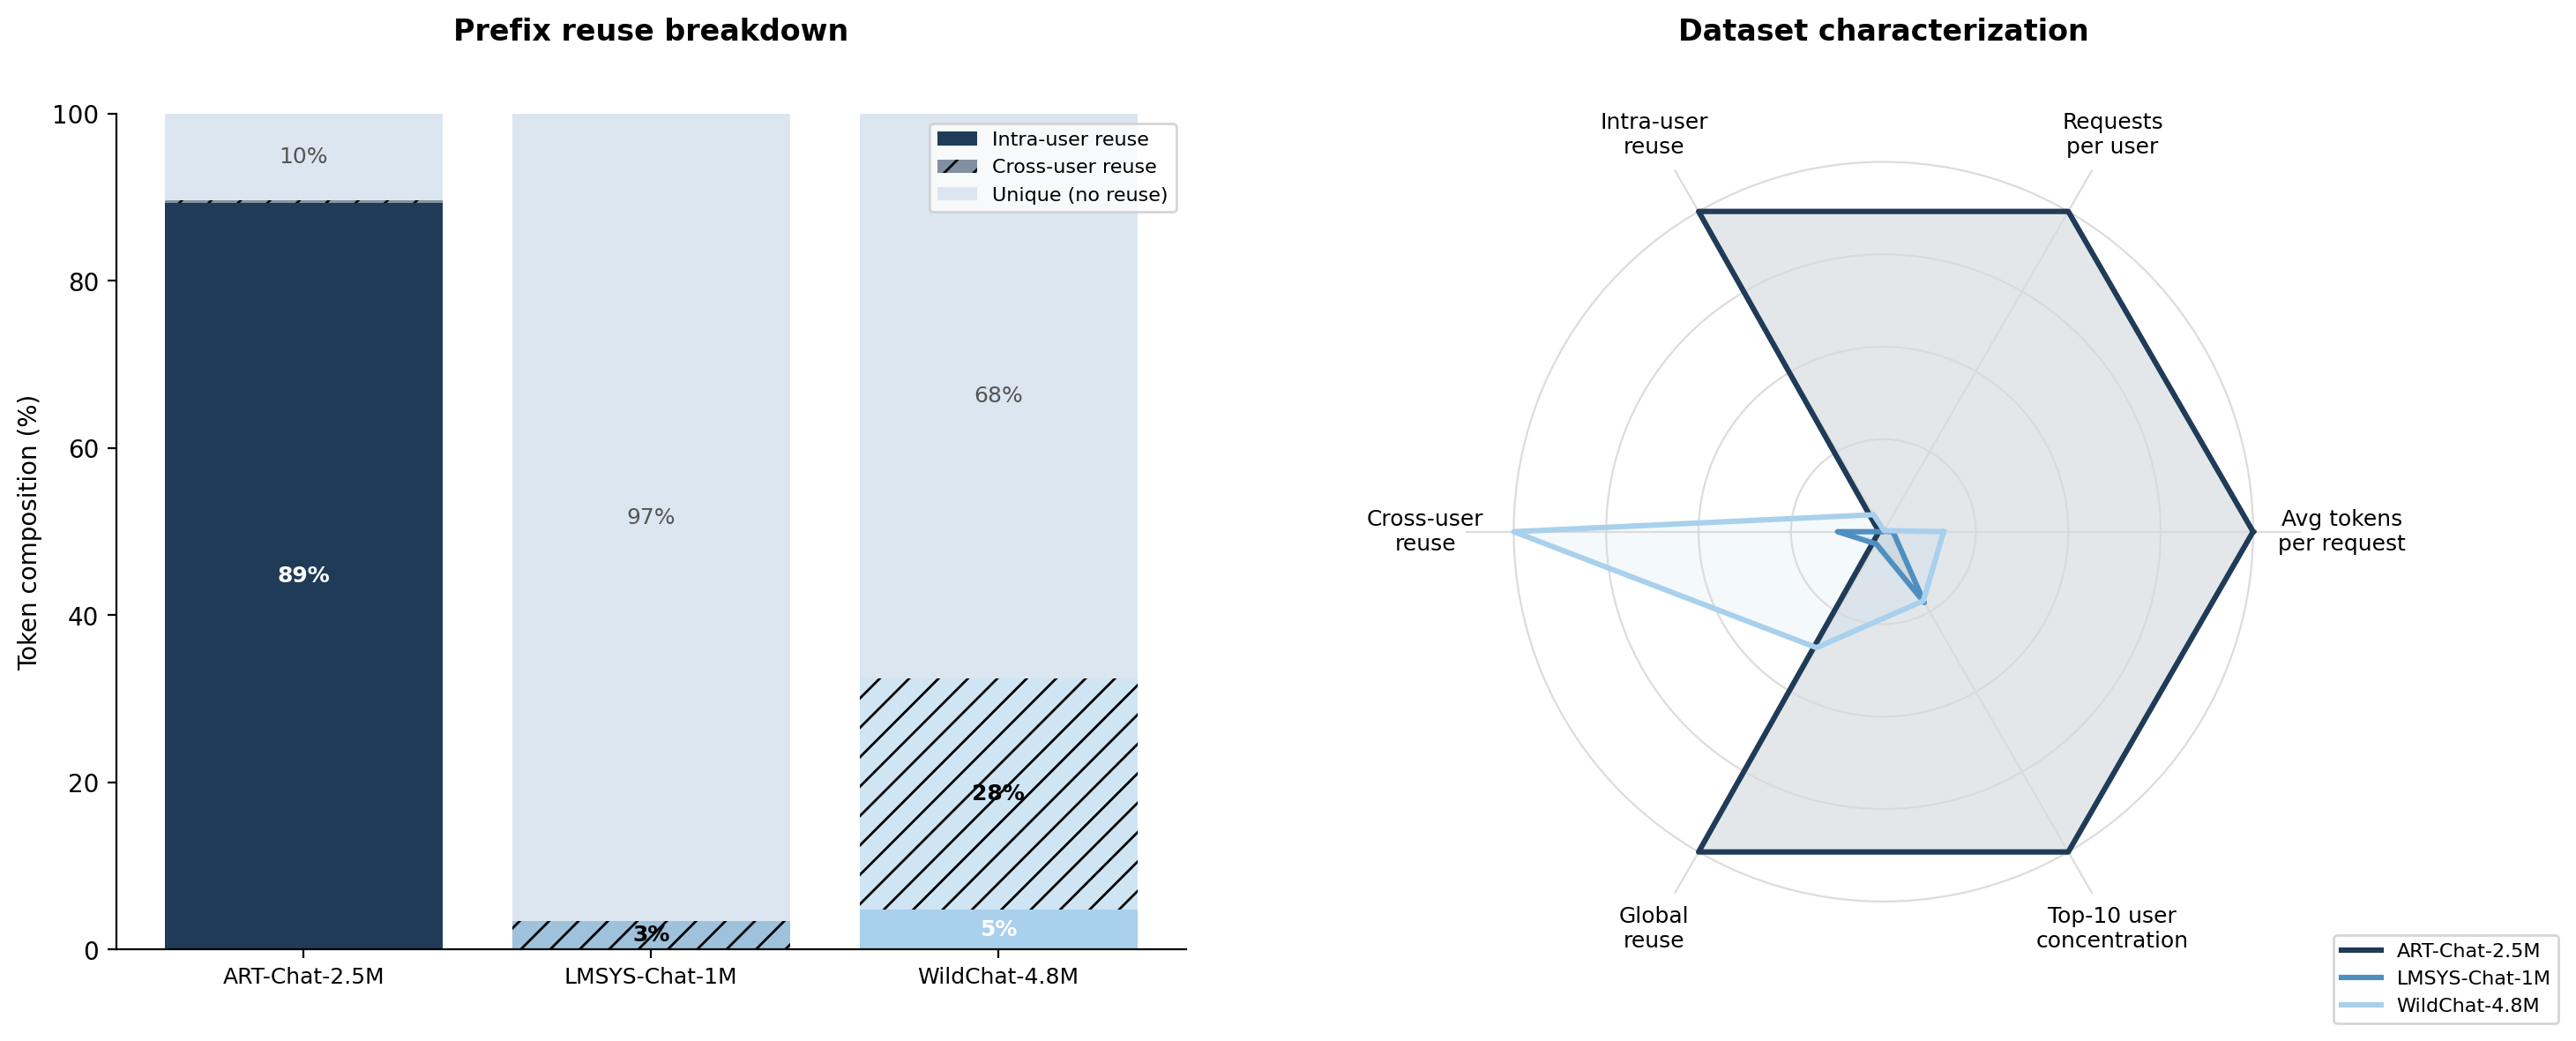
\includegraphics[width=\linewidth]{dataset_combined.png}
\caption{\textit{Left}: Dataset characterization. ART-Chat-2.5M's prefix reuse
  is overwhelmingly intra-user (89\%) with minimal cross-user reuse (0.3\%), which reflects
  the long-context, multi-turn data; WildChat's prefix reuse is predominantly cross-user (28\%, shared templates); LMSYS
  has minimal cross-user reuse (3\%) and no intra-user reuse due to the lack of a field for client origin. \textit{Right}: ART-Chat-2.5M
  contains the maximum for each attribute except for cross-user reuse, which in WildChat is a function of the shorter average token length (2,925 tokens) and a common system prompt.}
\label{fig:dataset_combined}
\end{figure}

% -----------------------------------------------------------------------
\FloatBarrier
\section{Experimental Setup}
\label{sec:setup}
% -----------------------------------------------------------------------

\paragraph{Proxy and engine configuration.}
Each policy runs the GORGO proxy on a small CPU worker in us-ashburn and controls
a dedicated SGLang inference engine in each of the following regions: us-ashburn,
eu-frankfurt, and ap-seoul. The engines contain two L40S GPUs each and serve the
Qwen3.5-35B-A3B model in FP8 format~\citep{qwen3technical}. All policies are
benchmarked on the same workload in parallel to rule out any variance in network
conditions. The round-trip time between the us-ashburn proxy and engines during
the tuning window is plotted in Figure~\ref{fig:rtt}. Due to the Qwen model's
limited context length of 32{,}768 tokens, we filter out any requests that
contain $>$24{,}000 tokens to leave adequate KV headroom. In SGLang, we set
\texttt{max\_concurrent\_requests} to 64 and \texttt{max\_output\_tokens} to 128
to limit unnecessary decode while simulating adequate load on the replica. All
workloads run alongside the proxy, dispatching requests to a local chat
completion endpoint.

\begin{figure}[t]
\centering
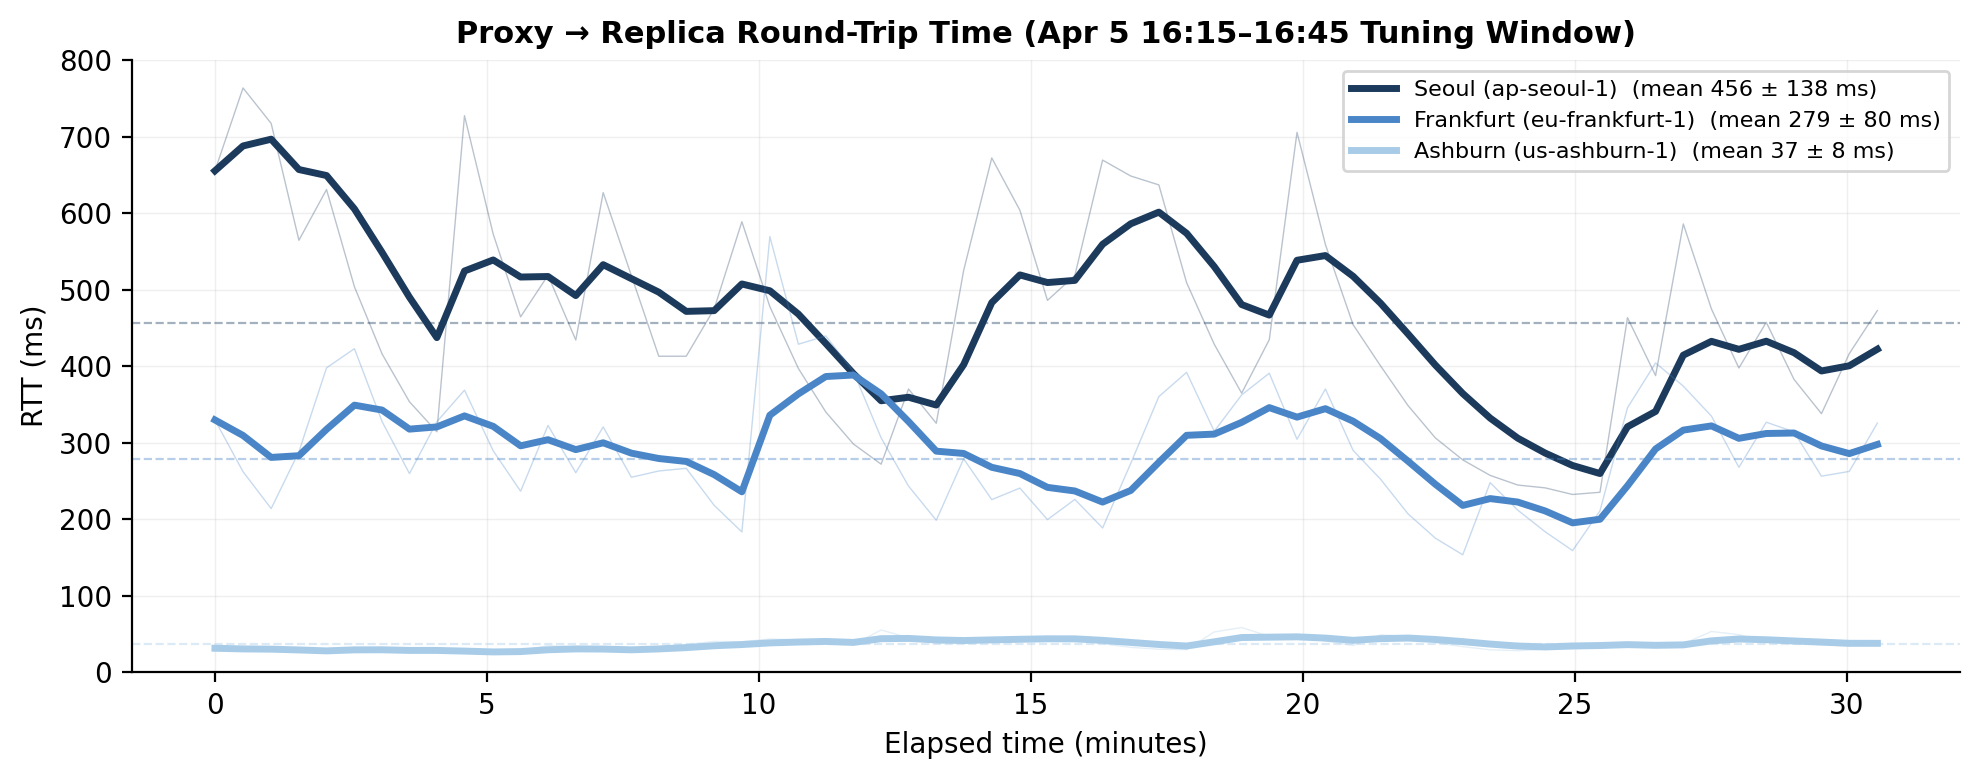
\includegraphics[width=\linewidth]{rtt_timeseries_apr5_1615_1645.png}
\caption{Round trip time (RTT) between the GORGO policy's proxy in us-ashburn and the SGLang engines in us-ashburn, eu-frankfurt, and ap-seoul
over the Apr~5 16:15--16:45 tuning window. The proxy measures RTT every 30 seconds on a separate probe from the \texttt{/metrics} request and smoothes the RTT with an exponential moving average (EWMA).
Each region's mean latency demonstrates that network latency either adds a consideration when choosing between replicas with disparate load and prefill cost or simplifies the choice when choosing between replicas with similar costs.}
\label{fig:rtt}
\end{figure}

\paragraph{Baseline policies.}
We benchmark the GORGO policy and compare performance of both online and static
modes to the below baselines. All SGLang metrics are scraped every 30 seconds
from the engine's Prometheus \texttt{/metrics} endpoint.
\begin{enumerate}
\item \texttt{least-load} minimizes the sum of proxy-tracked queued requests with
  SGLang metrics \texttt{num\_running\_reqs}, \texttt{num\_queue\_reqs}, and
  \texttt{num\_used\_tokens}. Queued requests to the proxy are defined as recently
  dispatched requests without a token response, and \texttt{num\_used\_tokens} are
  the currently occupied per-token KV slots.
\item \texttt{least-request} chooses the replica with the fewest in-flight
  requests from the proxy.
\item \texttt{prefix-cache} matches the request's prefix to the replica with the
  highest prefix-cache overlap, tracked on the proxy-side by a prefix trie of
  dispatched requests~\citep{aibrix2024}.
\item \texttt{simple-session-affinity} hashes the first 256 tokens from a request
  and routes to the replica with that prefix hash.
\end{enumerate}

\paragraph{Tuning and evaluation windows.}
We pick three 30-minute windows with high user diversity from the ART-Chat-2.5M
trace: Apr~5th 16:15--16:45, Apr~6 15:05--15:35, and Apr~7 19:45--20:15.
Statistics on each of these windows are found in Table~\ref{tab:windows}
(Appendix~\ref{app:windows}). We
assign Apr~5th as the window where we tune GORGO's weights online to minimize the
p95 TTFT of a rolling 128-request window with hop size 32. $w_{\mathrm{rtt}}$ and
$w_{\mathrm{queue}}$ are each initialized to 0.5 and 0.1 and restricted to ranges
$[0.05, 2.0]$ and $[0.05, 0.5]$. These values are hand-picked from the paradigm
of continuous batching in SGLang, where incoming requests can be scheduled into
the current batch, affecting TTFT less significantly than a fixed floor of
network latency between regions. The Apr~6--7 windows fix weight values GORGO
learned on the Apr~5 tuning window. Due to the greater number of requests in
Apr~6--7, we increase \texttt{time\_scale} to 2.0 and 3.0, respectively, to
control replica saturation (Table~\ref{tab:loadsweep}).

% -----------------------------------------------------------------------
\FloatBarrier
\section{Results}
\label{sec:results}
\label{sec:results:p95}
% -----------------------------------------------------------------------


\paragraph{Results across three windows.}

\begin{table}[htbp]
\centering
\small
\caption{Experiment results. In the tuning window, GORGO learns weights $w_{\mathrm{rtt}}{=}0.276$, $w_{\mathrm{queue}}{=}0.5$ after initializing
at weights $w_{\mathrm{rtt}}{=}0.5$, $w_{\mathrm{queue}}{=}0.1$. On held out evaluation windows, GORGO's weights are frozen, and
the policy outperforms every baseline policy on P95 TTFT.}
\label{tab:results}
\setlength{\tabcolsep}{2.7pt}
\begin{tabular}{lrrrrrrr}
\toprule
Policy & TTFT P50 (ms) & TTFT P95 & TTFT P99 & E2E P50 (s) & E2E P95 & E2E P99 & ITL (ms) \\
\midrule
\multicolumn{8}{l}{\textit{Tuning window --- Apr~5 16:15--16:45 (time\_scale${=}1.0$, 7{,}195 requests)}} \\
\midrule
\textbf{GORGO}          & \textbf{673} & 2{,}514          & 4{,}473          & \textbf{3.04}  & \textbf{8.91}  & \textbf{17.54} & \textbf{17.6} \\
simple-session-affinity & 712          & \textbf{2{,}428} & 5{,}190          & 3.48           & 18.27          & 22.61          & 20.2 \\
least-load              & 763          & 2{,}447          & \textbf{4{,}349} & 3.63           & 13.69          & 17.57          & 21.7 \\
least-request           & 968          & 3{,}970          & 7{,}012          & 4.37           & 16.62          & 20.81          & 25.2 \\
prefix-cache            & 1{,}477      & 6{,}784          & 9{,}613          & 13.14          & 22.63          & 26.81          & 82.3 \\
\midrule
\multicolumn{8}{l}{\textit{Held-out eval --- Apr~6 15:05--15:35 (time\_scale${=}2.0$, 7{,}630 requests)}} \\
\midrule
\textbf{GORGO}          & \textbf{491} & \textbf{1{,}584} & \textbf{2{,}222} & \textbf{1.80}  & \textbf{3.28}  & \textbf{4.37}  & \textbf{9.0} \\
simple-session-affinity & 627          & 1{,}875          & 3{,}056          & 2.01           & 4.75           & 7.34           & 10.3 \\
least-load              & 616          & 1{,}818          & 2{,}885          & 2.17           & 4.06           & 5.78           & 10.7 \\
least-request           & 634          & 1{,}852          & 2{,}484          & 2.08           & 3.99           & 5.23           & 9.9 \\
prefix-cache            & 574          & 1{,}798          & 2{,}750          & 2.07           & 4.95           & 10.34          & 10.6 \\
\midrule
\multicolumn{8}{l}{\textit{Held-out eval --- Apr~7 19:45--20:15 (time\_scale${=}3.0$, 8{,}663 requests)}} \\
\midrule
\textbf{GORGO}          & \textbf{398} & \textbf{1{,}417} & \textbf{2{,}061} & \textbf{1.74}  & \textbf{3.36}  & 6.81           & \textbf{9.3} \\
simple-session-affinity & 457          & 1{,}522          & 2{,}402          & \textbf{1.74}  & 3.92           & 7.12           & \textbf{9.3} \\
least-load              & 495          & 1{,}669          & 2{,}368          & 1.95           & 4.07           & \textbf{6.22}  & 10.0 \\
least-request           & 527          & 1{,}759          & 2{,}578          & 1.98           & 4.44           & 7.85           & 10.0 \\
prefix-cache            & 533          & 1{,}861          & 2{,}872          & 2.20           & 12.00          & 20.04          & 11.8 \\
\bottomrule
\end{tabular}
\end{table}

Table~\ref{tab:results} reports TTFT, E2E latency, and inter-token latency (ITL)
for all policies in all three windows. While the GORGO policy's weights are
updated to minimize p95 TTFT during tuning, the held-out, fixed-weight evaluation
shows generalization of the learned values across days, with GORGO improving p95
TTFT by 6.9--15.5\% and E2E latency by 14.3--30.9\% over session-affinity. GORGO
slightly underperforms baseline policies on the tuning window because the
evolutionary strategy actively explores the space of parameters and tests worse weights than the learned solution, which converges after 672 samples
(Figure~\ref{fig:es_convergence}).

\begin{figure}[htbp]
\centering
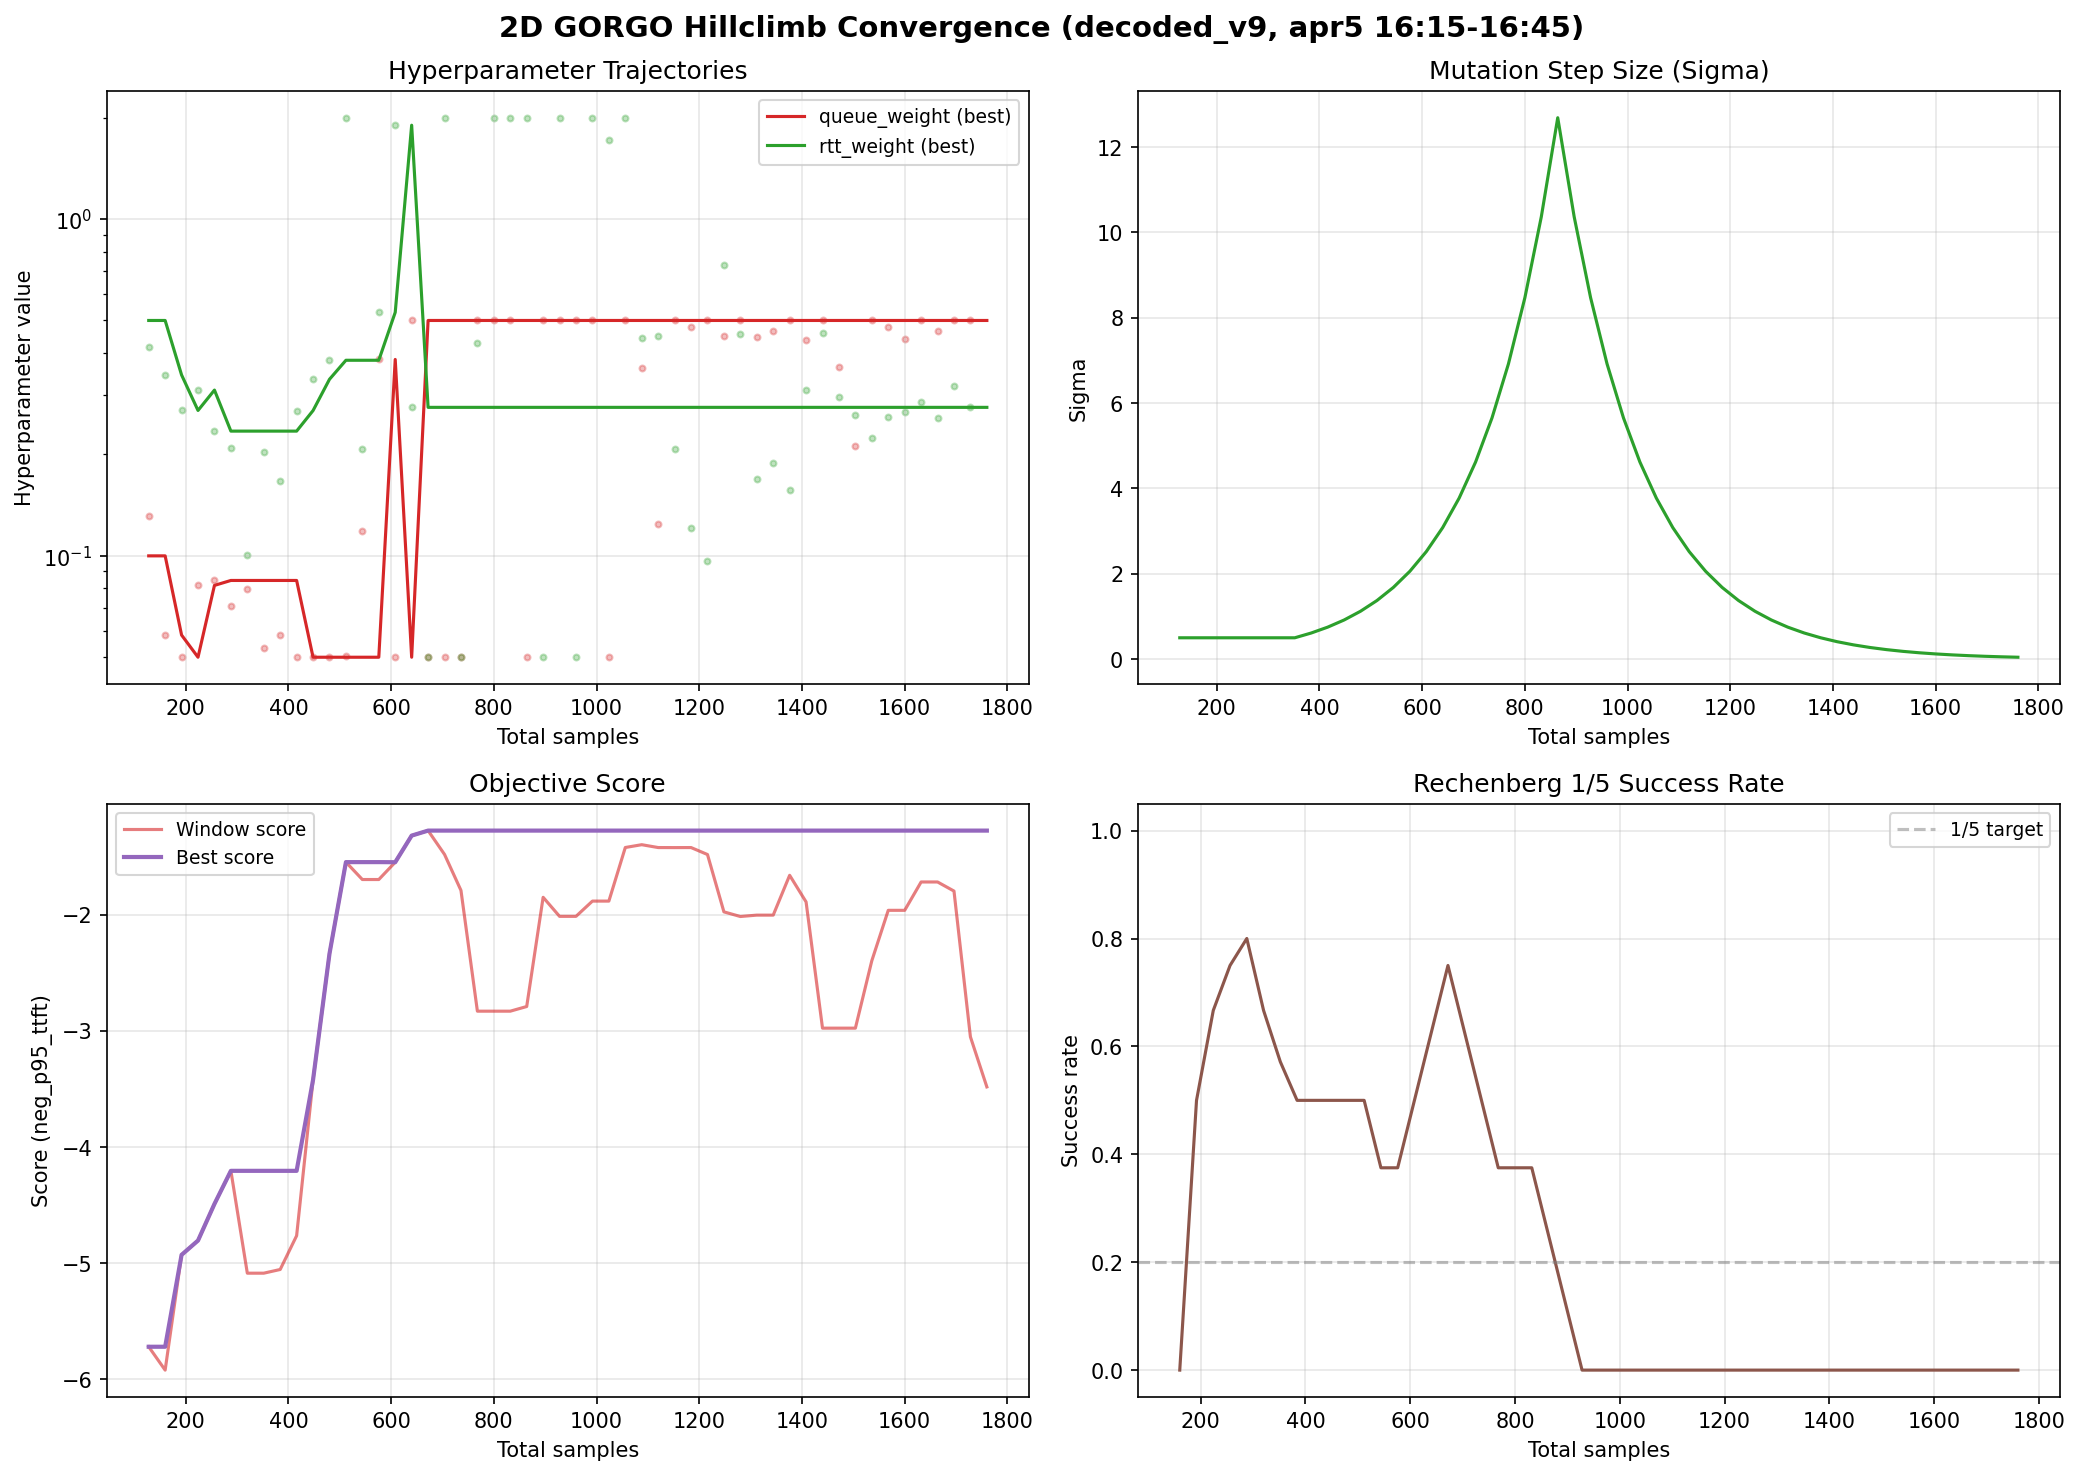
\includegraphics[width=\linewidth]{tune_convergence_2d_v9.png}
\caption{Convergence of the evolutionary strategy on GORGO policy weights $w_{\mathrm{queue}}$ and $w_{\mathrm{rtt}}$.
Both weights reach their local optima after 672 samples, which occurs on the 18th evolutionary step. The best objective
score on this window is -1.276 P95 TTFT. This metric is negative due to the evolutionary strategy's objective of maximizing negative P95 TTFT, which is the fitness function.}
\label{fig:es_convergence}
\end{figure}

% -----------------------------------------------------------------------
\paragraph{Load Sweep}

We find when sweeping across the \texttt{time\_scale} parameter that our SGLang inference engines reach a saturation point. After a concurrency threshold is reached,
requests begin to experience HOL queueing delay. In Table~\ref{tab:loadsweep}, the policies experience a 3$\times$ improvement in P95 TTFT and P95 E2E latency after \texttt{time\_scale=3.0} is reached.
In the tuning window, most policies other than GORGO are over saturating replicas due to the abnormally high P95 E2E latency when compared to the P95 E2E latency in later windows.
We recommend sweeping across timescales to find a clean under-saturated traffic profile before running GORGO. Due to the increased load profile of Apr 6-7, the timescale was increased to create a fair evaluation environment. However, we include in Appendix~\ref{app:apr7_ts2} a reference run of Apr~7 with \texttt{time\_scale}${=}2.0$ to show saturation at a lower timescale.

\begin{table}[htbp]
\centering
\small
\setlength{\tabcolsep}{4.5pt}
\caption{Load sweep. A sweep of the timescale variable, which linearly scales the time between requests, shows
P95 TTFT and E2E latency degrading at lower timescales. After \texttt{time\_scale${=}3.0$}, metrics improve by over 3$\times$ for unsaturated policies. Notably,
this timescale sweep shows that GORGO breaks the saturation point earlier than other policies due to a well-tuned load term.}
\label{tab:loadsweep}
\begin{tabular}{lrrrc}
\toprule
Policy & Input & TTFT P95 & E2E P95 & Saturated? \\
       & (tok/s) & (ms)     & (s)     &            \\
\midrule
\multicolumn{5}{l}{\textit{time\_scale${=}1.0$ (full load)}} \\
\midrule
gorgo                   & 34{,}064 & 8{,}260 & 15.76 & yes \\
simple-session-affinity & 34{,}035 & 1{,}835 & 17.94 & yes \\
least-request           & 34{,}030 & 6{,}138 & 18.62 & yes \\
\midrule
\multicolumn{5}{l}{\textit{time\_scale${=}2.0$}} \\
\midrule
gorgo                   & 17{,}003 & 1{,}822 & 5.65  & no  \\
simple-session-affinity & 16{,}999 & 1{,}707 & 15.50 & yes \\
least-request           & 16{,}999 & 4{,}361 & 16.85 & yes \\
\midrule
\multicolumn{5}{l}{\textit{time\_scale${=}3.0$}} \\
\midrule
gorgo                   & 11{,}327 & 1{,}378 & 3.25  & no  \\
simple-session-affinity & 11{,}326 & 1{,}556 & 4.04  & no  \\
least-request           & 11{,}326 & 1{,}805 & 4.92  & no  \\
\bottomrule
\end{tabular}
\end{table}

\paragraph{Exploiting Continuous Batching in SGLang}
\label{sec:results:hacking}
In the continuous batching paradigm, we learned that GORGO can stumble upon abnormal weight values and achieve an impressively low P95 TTFT at the cost of high P95 E2E latency.
Appendix~\ref{app:load_ablation} presents results from an experiment where the evolutionary strategy learns to set $w_{\mathrm{queue}}$
to 0 while keeping $w_{\mathrm{rtt}}$ near 0.23, which results in P95 TTFT 17\% better than the next-best policy. For this window,
GORGO chose to send 100\% of requests to the closest replica in us-ashburn. Continuous batching~\citep{orca2022} works by admitting incoming requests into the currently
running batch as long as some concurrency slot exists for the request. Thus, when all requests are sent to the same replica, any new requests sent to that replica can enter the batch, reuse existing KV-cache,
and prefill a single token. However, once the request enters the memory-bound decode phase, the replica's memory headroom saturates, KV-cache thrashes between GPU and CPU memory, and ITL/E2E latency collapses~\citep{orca2022, vllm2023}. 



% -----------------------------------------------------------------------

\section{Related Work}
\label{sec:related}
% -----------------------------------------------------------------------

\paragraph{Prefix caches and reuse.}
RadixAttention in SGLang \citep{sglang2024} stores per-request KV state in a
radix tree; PagedAttention in vLLM \citep{vllm2023} enables prefix sharing
through paged memory. KVLink \citep{kvlink2025}, ChunkKV \citep{chunkkv2025},
KVFlow \citep{kvflow2025}, and Learned Prefix Caching \citep{lpc2025} improve
the single-replica cache but do not decide which replica serves a request.

\paragraph{Cross-replica routing and cross-region serving.}
Preble \citep{preble} introduces longest-prefix-match routing across replicas
with a load-balance fallback; AIBrix \citep{aibrix2024} packages a
production-grade variant of the same design and supplies the baseline we run.
Mooncake \citep{qin2024mooncake} is a KV-cache-centric architecture and the
source of our trace format. SkyServe \citep{skyserve} and SkyWalker
\citep{skywalker} address cross-region LLM serving at the placement and
spillover layers respectively, but treat per-request routing as out of scope.
k-LPM \citep{klpm2025} formulates LLM scheduling under TTFT constraints as
NP-hard. DLPM \citep{dlpm2025} targets fairness with locality. Llumnix
\citep{llumnix2024} migrates requests across replicas. Multi-LLM routers
\citep{routerwu2025} address model selection. CacheBlend
\citep{yao2024cacheblend} routes by trie-measured prefix length but does not
measure network RTT. DistServe \citep{distserve2024} and Splitwise
\citep{splitwise2024} disaggregate prefill from decode. GORGO is the first
single-router policy in this space that scores cache locality, replica load,
and wide-area latency in one cost and derives the cost weights from the
deployment's own per-request TTFT stream, with no engine modifications.

\paragraph{Online hyperparameter adaptation.}
Bayesian and bandit-based methods have been applied to serving configuration
\citep{routerwu2025}. For a 2-dimensional parameter space the $(1{+}1)$-ES
\citep{rechenberg1973} provides fast, overhead-free convergence with no
surrogate model.

% -----------------------------------------------------------------------
\section{Conclusion}
\label{sec:conclusion}
% -----------------------------------------------------------------------

Routing across LLM replicas is a three-signal decision balancing cache locality, replica
load, and wide-area latency, but production heuristics commit to one signal and
degrade when that stops being the limiting factor. We treat the three as
terms of an additive per-replica cost and let online TTFT feedback optimize 
scaling weights, in place of operator-tuned constants or offline profiling. On a
long-context, high-prefix-reuse production trace the GORGO policy family
collectively achieves the lowest TTFT at every reported percentile in both a
tuning and a held-out evaluation windows. On a short-prompt, low-reuse public
trace (Appendix~\ref{app:wildchat}) the same policy is non-competitive, in
agreement with the regime characterization in
\S\ref{sec:characterization}. The advantage is therefore a property of the
workload regime as much as of the policy: it scales with how much of TTFT is
recoverable through prefill reuse, queue avoidance, or network selection rather
than fixed by hardware. The design choices of GORGO transfer to
deployments where the workload regime is not known in advance and a dedicated
calibration window before each redeploy is not affordable, making it effective in production LLM serving on long context, distributed workloads. 

\bibliographystyle{plainnat}
\bibliography{references}

\newpage

\section*{NeurIPS Paper Checklist}

\begin{enumerate}

\item {\bf Claims}\\
Question: Do the main claims made in the abstract and introduction accurately reflect the paper's contributions and scope?\\
Answer: \answerYes{}\\
Justification: The abstract claims (i) public datasets underrepresent long-context multi-turn traffic (quantified in \S\ref{sec:characterization}), (ii) we evaluate routing policies on a production trace (Table~\ref{tab:results}), and (iii) GORGO sweeps every TTFT percentile on the held-out windows. We are explicit in the introduction, \S\ref{sec:results:p95}, and \S\ref{sec:limitations} that ``GORGO'' refers to a family, that the W2 p99 margin is at the noise floor, and that on the daytime stress window \texttt{gorgo-hillclimb}'s p99 inflates and \texttt{prefix-cache} wins p99 instead.

\item {\bf Limitations}\\
Question: Does the paper discuss the limitations of the work?\\
Answer: \answerYes{}\\
Justification: Section~\ref{sec:limitations} lists single-trace generalization, the W2 p99 noise floor, the single-tenant assumption, \texttt{gorgo-autotune} instability, hardware homogeneity, the absence of PD-disaggregation, and ES convergence time.

\item {\bf Theory assumptions and proofs}\\
Question: For each theoretical result, does the paper provide the full set of assumptions and a complete proof?\\
Answer: \answerNA{}\\
Justification: The paper presents an additive cost model and an online optimizer with no formal theorems.

\item {\bf Experimental result reproducibility}\\
Question: Does the paper fully disclose all the information needed to reproduce the main experimental results?\\
Answer: \answerYes{}\\
Justification: Section~\ref{sec:setup} specifies model, regions, hardware, fleet topology, concurrency, trace windows, and per-window GORGO seeding. Section~\ref{sec:method} gives Equation~\ref{eq:score}, the $(1{+}1)$-ES configuration ($\sigma_0=0.5$, 1/5-rule, hop 16, window 64), and the median-of-rates fit. 
% The reproducibility statement enumerates four canonical paths in the released artifact.

\item {\bf Open access to data and code}\\
Question: Does the paper provide open access to the data and code?\\
Answer: \answerYes{}\\
Justification: The proxy and policy code are available at \href{https://anonymous.4open.science/r/GORGO-D25A}{https://anonymous.4open.science/r/GORGO-D25A}. The ART-Chat-2.5M trace is not redistributable under its terms of service. The public-dataset characterization (LMSYS, WildChat) is fully reproducible with no proprietary inputs.

\item {\bf Experimental setting/details}\\
Question: Does the paper specify all the training and test details?\\
Answer: \answerYes{}\\
Justification: Section~\ref{sec:setup} specifies model, hardware, regions, concurrency, trace windows, max input tokens, and per-window seeding for adaptive policies. ES configuration is given in Section~\ref{sec:method}.

\item {\bf Experiment statistical significance}\\
Question: Does the paper report error bars or appropriate statistical significance information?\\
Answer: \answerYes{}\\
Justification: Section~\ref{sec:limitations} derives an approximate p99 standard error and shows that the W2 p99 margin between \texttt{gorgo-hillclimb} and \texttt{random} is inside one standard error, while the W1 sweep and W2 p50/p95 wins are several standard errors clear of zero.

\item {\bf Experiments compute resources}\\
Question: Does the paper provide sufficient information on compute resources?\\
Answer: \answerYes{}\\
Justification: Each policy runs on a dedicated 3-replica fleet of L40S SGLang servers (tensor-parallel 2, 96\,GB VRAM per replica). Eight policies $\times$ two windows $= 16$ fleet-runs, each $\sim$30 min wall clock, on three regions. Total GPU-hours: $\approx$24.

\item {\bf Code of ethics}\\
Question: Does the research conform with the NeurIPS Code of Ethics?\\
Answer: \answerYes{}\\
Justification: The work concerns routing infrastructure. The production trace is used under terms that permit research replay; we release only aggregated prefix-trie statistics, not individual requests. No individuals are identifiable from the released aggregates.

\item {\bf Broader impacts}\\
Question: Does the paper discuss potential societal impacts?\\
Answer: \answerYes{}\\
Justification: Routing improvements reduce the energy and dollar cost of serving LLMs at fixed quality. Lower-cost serving may accelerate deployment in settings where that is socially harmful; the contributions are infrastructure-level and do not affect model capability.

\item {\bf Safeguards}\\
Question: Does the paper describe safeguards for responsible release?\\
Answer: \answerNA{}\\
Justification: We do not release datasets or models. The released code is a routing proxy and policy library with no inherent dual-use beyond LLM-serving infrastructure.

\item {\bf Licenses}\\
Question: Are creators or owners of assets properly credited?\\
Answer: \answerYes{}\\
Justification: SGLang, vLLM, AIBrix, LMSYS-Chat-1M, WildChat-4.8M, and Qwen3 are cited and used under their published licenses.

\item {\bf New assets}\\
Question: Are new assets introduced in the paper well documented?\\
Answer: \answerYes{}\\
Justification: The proxy, policy library, experiment controller, and trace builder are documented in the repository's top-level documentation. Spec and manifest files are stored alongside the controller.

\item {\bf Crowdsourcing and research with human subjects}\\
Question: Does the paper involve crowdsourcing or human subjects?\\
Answer: \answerNA{}\\
Justification: No human subjects.

\item {\bf IRB approvals}\\
Answer: \answerNA{}\\
Justification: No human subjects.

\item {\bf Declaration of LLM usage}\\
Question: Does the paper describe the usage of LLMs if it is an important, original, or non-standard component of the research methodology?\\
Answer: \answerNA{}\\
Justification: LLM serving infrastructure is the object of study. Authors used LLMs for routine writing assistance only.

\end{enumerate}

\newpage

% \section*{Reproducibility Statement}

% The experiments are driven by a single experiment controller that launches fleets,
% configures policies, and replays a trace per policy. The four canonical paths in
% the released artifact are:

% \begin{itemize}
% \item \path{specs/policy_matrix_abstract_night.json} --- W1 spec (eight policies, manual GORGO starter weights);
% \item \path{specs/policy_matrix_abstract_night_w2.json} --- W2 spec (eight policies, GORGO seeded with W1-learned weights);
% \item \path{experiment_runner/policy_matrix_app.py} --- experiment controller;
% \item \path{data_processing/build_mooncake_trace.py} --- trace builder.
% \end{itemize}

% W1 and W2 manifests, result CSVs, and summary plots are produced by running the
% controller against these specs and post-processing per-policy stats with the
% released analysis scripts. The ART-Chat-2.5M trace is not redistributable;
% the public-dataset characterization (LMSYS, WildChat) reproduces with no
% proprietary inputs.

\appendix

\section{Evaluation Window Characteristics}
\label{app:windows}

Table~\ref{tab:windows} characterizes the three decoded replay windows used in
\S\ref{sec:setup} and Table~\ref{tab:results}.

\begin{table}[h]
\centering
\small
\caption{Workload characteristics of the three decoded replay windows in
  Table~\ref{tab:results}. Users, requests-per-user, token lengths, and block
  reuse are measured on the decoded replay files actually benchmarked; block
  reuse is token-weighted 256-token global / intra-user prefix reuse. Turn
  structure ($\dagger$) is measured on the source window metadata and is
  preserved by the synthetic decode. Token counts use tiktoken gpt-4o.}
\label{tab:windows}
\begin{tabular}{lrrr}
\toprule
 & Apr5 tuning & Apr6 eval & Apr7 eval \\
 & 16:15--16:45 & 15:05--15:35 & 19:45--20:15 \\
 & time\_scale 1.0 & time\_scale 2.0 & time\_scale 3.0 \\
\midrule
Distinct users               & 579      & 606      & 540      \\
Requests / user              & 12.8     & 12.9     & 16.4     \\
Avg turns / conv.$^\dagger$  & 30.3     & 27.7     & 21.5     \\
Multi-turn requests$^\dagger$ & 73.9\%  & 74.1\%   & 73.7\%   \\
Median input tokens          & 5{,}638  & 5{,}787  & 5{,}745  \\
Avg input tokens             & 6{,}877  & 7{,}008  & 7{,}148  \\
p95 input tokens             & 19{,}886 & 20{,}974 & 20{,}435 \\
Block global reuse           & 78.8\%   & 77.6\%   & 87.9\%   \\
Block intra-user reuse       & 78.5\%   & 77.1\%   & 87.4\%   \\
\bottomrule
\end{tabular}
\end{table}

\section{Apr~7 at \texttt{time\_scale}${=}2.0$ (saturation reference)}
\label{app:apr7_ts2}

The main held-out evaluation replays Apr~7 at \texttt{time\_scale}${=}3.0$
because at \texttt{time\_scale}${=}2.0$ the concentrating and cache-blind
baselines are past their saturation knee. Table~\ref{tab:apr7_ts2} reports the
full 5-policy run at \texttt{time\_scale}${=}2.0$ ($n{=}8{,}663$ per policy).
\texttt{simple-session-affinity} posts the best TTFT at every percentile, yet its
E2E p95 is 14.66\,s versus GORGO's 7.10\,s, and \texttt{prefix-cache} melts
(E2E p95 22.14\,s, client scheduling-slip p95 $\sim$181\,s): continuous batching
admits the first token on schedule even on a saturated replica, so TTFT looks
healthy while E2E exposes the overload. GORGO holds the lowest E2E at this load
but trails on TTFT---a saturation artifact, not a routing deficit---which is why
the clean within-capacity comparison in Table~\ref{tab:results} uses
\texttt{time\_scale}${=}3.0$.

\begin{table}[h]
\centering
\small
\setlength{\tabcolsep}{2.7pt}
\caption{Apr~7 19:45--20:15 held-out window at \texttt{time\_scale}${=}2.0$
  (5 policies, $n{=}8{,}663$ each). ITL is the median inter-token latency. Bold is
  best in column. TTFT looks best for the concentrating baselines while E2E
  reveals their saturation.}
\label{tab:apr7_ts2}
\begin{tabular}{lrrrrrrr}
\toprule
Policy & TTFT p50 (ms) & TTFT p95 & TTFT p99 & E2E p50 (s) & E2E p95 & E2E p99 & ITL (ms) \\
\midrule
GORGO                   & 586          & 1{,}891          & 3{,}431          & 2.38          & \textbf{7.10}  & \textbf{12.58} & 13.4 \\
simple-session-affinity & \textbf{512} & \textbf{1{,}684} & \textbf{2{,}455} & \textbf{2.19} & 14.66          & 17.19          & \textbf{12.2} \\
least-load              & 633          & 2{,}158          & 3{,}753          & 2.69          & 10.39          & 16.19          & 15.5 \\
least-request           & 915          & 4{,}806          & 7{,}114          & 3.77          & 17.27          & 19.61          & 19.7 \\
prefix-cache            & 1{,}474      & 8{,}243          & 12{,}167         & 7.67          & 22.14          & 26.66          & 45.7 \\
\bottomrule
\end{tabular}
\end{table}

\section{WildChat replay (regime-sensitivity control)}
\label{app:wildchat}

We replay a 30-minute window of WildChat-4.8M \citep{wildchat2024} on the
same 2$\times$L40S three-region fleet, with the same seven policies as the
ART-Chat-2.5M sweeps (five baselines plus \texttt{gorgo (online)} and
\texttt{gorgo (fixed)}). WildChat averages 2{,}925 input tokens per request and
4.7\% intra-user prefix reuse---an order of magnitude shorter than ART-Chat-2.5M
and a small fraction of the reuse---putting it well outside the regime
characterized in \S\ref{sec:characterization}.

\begin{table}[h]
\centering
\small
\caption{WildChat-4.8M replay: 30-minute window, $c{=}32$. TTFT in seconds.
  Bold is best in column. Compared to the ART-Chat-2.5M results, GORGO variants
  are not competitive: \texttt{gorgo (fixed)} is the slowest policy on p95.}
\label{tab:wildchat}
\begin{tabular}{lrrrrrr}
\toprule
Policy & Completed & p50 & p95 & p99 & max & Succ.\% \\
\midrule
\textbf{simple-session-affinity} & 20{,}447 & 0.416 & \textbf{1.025} & \textbf{1.712} & 7.75    & 99.6 \\
least-request                    & 20{,}517 & 0.480 & 1.036          & 1.731          & 110.45  & 100.0 \\
random                           & 20{,}436 & \textbf{0.416} & 1.077 & 1.796          & 15.82   & 99.6 \\
prefix-cache                     & 20{,}504 & 0.497 & 1.186          & 2.588          & 10.63   & 99.9 \\
least-load                       & 20{,}484 & 0.532 & 1.217          & 2.535          & 8.28    & 99.8 \\
gorgo (online)                   & 20{,}473 & 0.541 & 1.325          & 2.654          & 7.05    & 99.8 \\
gorgo (fixed)                    & 20{,}462 & 0.709 & 1.932          & 3.969          & 60.18   & 99.7 \\
\bottomrule
\end{tabular}
\end{table}

\begin{figure}[h]
\centering
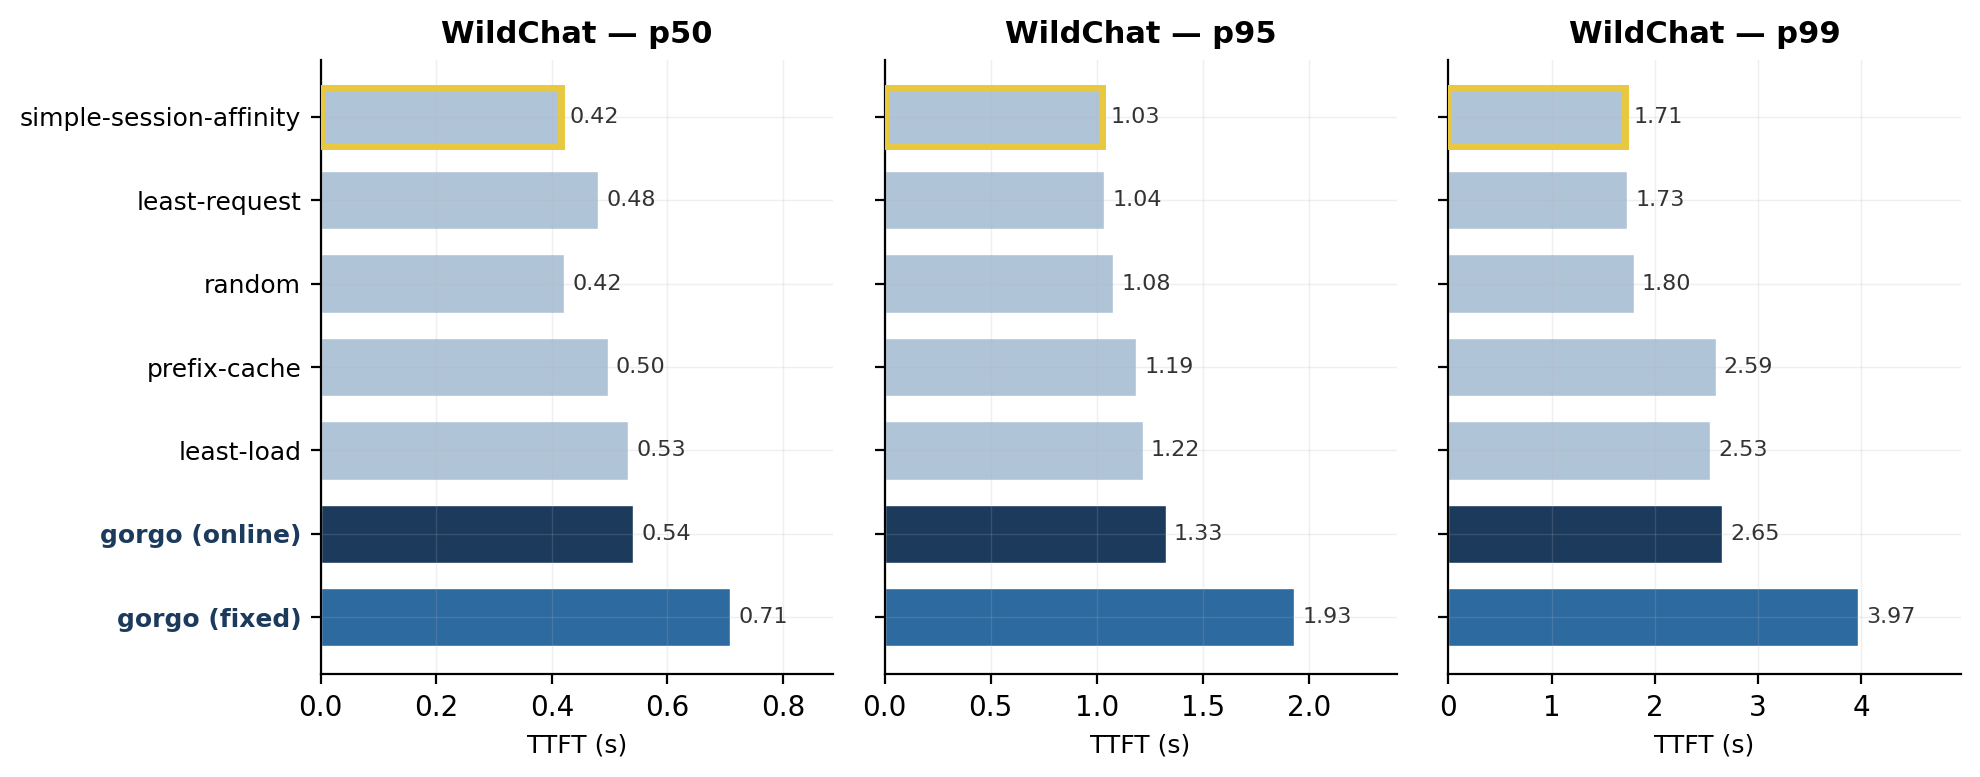
\includegraphics[width=\linewidth]{ttft_bars_wildchat.png}
\caption{WildChat-4.8M replay, per-percentile TTFT (p50/p95/p99) across
  the seven policies. GORGO variants (dark blues) are not competitive:
  \texttt{gorgo (fixed)} is the slowest policy at the tail, and
  \texttt{gorgo (online)} sits mid-pack. The ranking inverts the
  ART-Chat-2.5M result, consistent with the regime argument in
  \S\ref{sec:characterization}.}
\label{fig:ttft_bars_wildchat}
\end{figure}

The ranking is reversed: \texttt{simple-session-affinity} wins p95 and
p99 by a large margin, \texttt{least-request} is competitive,
\texttt{gorgo (online)} sits mid-pack, and \texttt{gorgo (fixed)} is the
slowest policy. Two mechanisms drive this. First, the prefill term in
Equation~\ref{eq:score} is small at 2{,}925 tokens; the cost-model weights
are mostly fitting noise. Second, intra-user reuse is 4.7\% rather than
89\%; even a perfect cache-routing decision saves only a few hundred tokens
per request, well inside the cross-region RTT band, so chasing cache
locality is counterproductive when paired with a cross-region routing
penalty. The \texttt{gorgo (fixed)} weights frozen from an ART-Chat-2.5M W1
are particularly mis-calibrated to this regime---a reminder that the
cost-model parameters do not transfer across workload classes.

We include this result as a regime-sensitivity control, not as a
contribution. The takeaway is the same one stated in \S\ref{sec:characterization}:
the gain from joint cache--network--queue routing depends on the workload
having long prompts and substantial intra-user prefix reuse. Public chat
datasets do not exercise this regime.

\section{GORGO Achieves Convergence of Cache Reuse}
\label{app:convergence}

\begin{figure}[h]
\centering
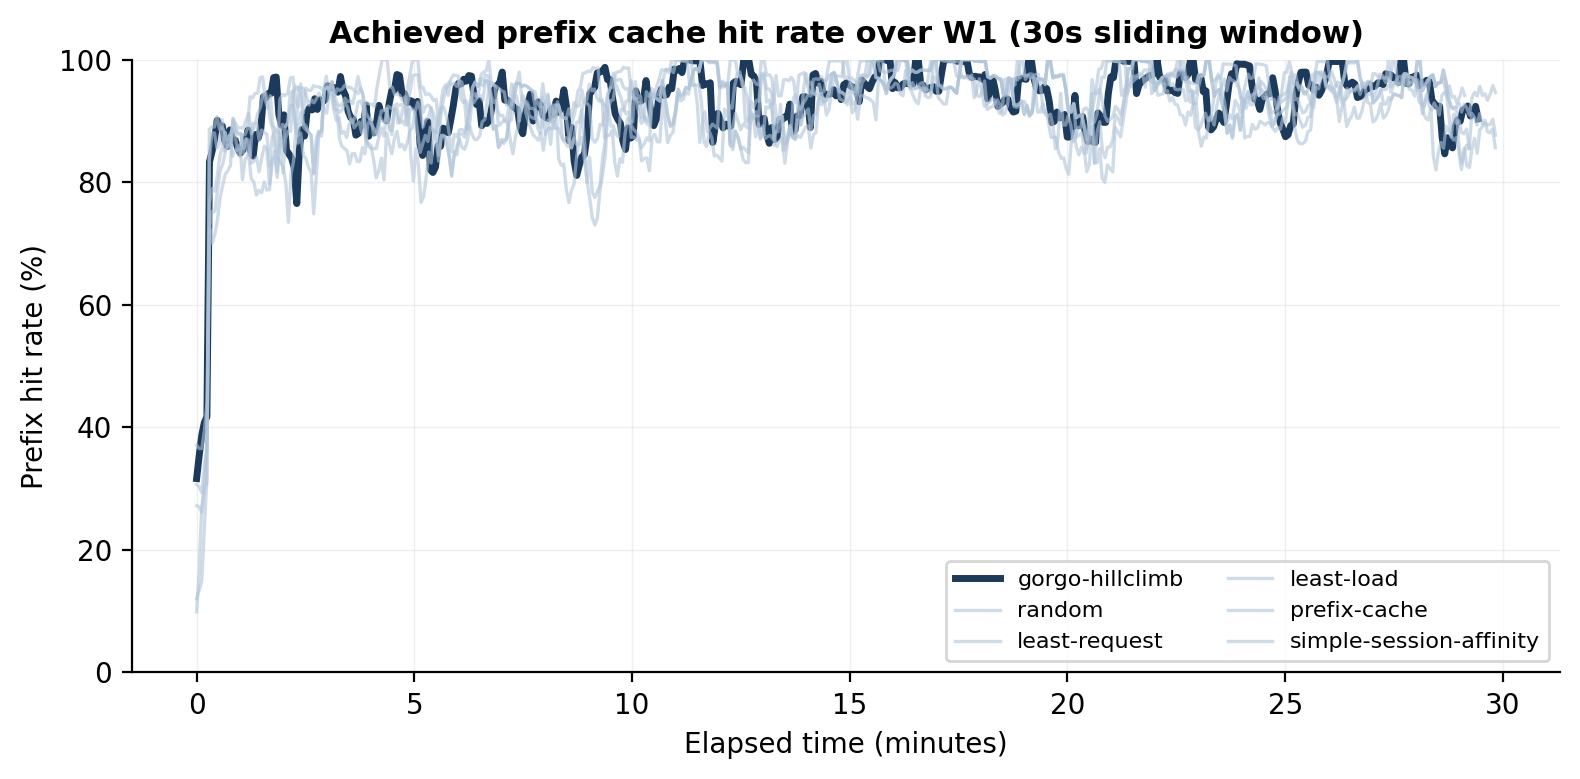
\includegraphics[width=0.75\linewidth]{cache_convergence.png}
\caption{Achieved prefix hit rate over the W1 tuning window: the fraction
  of each request's input tokens that were already cached on the replica
  the policy routed to (not the total cache available across all replicas).
  A higher rate means the routing decision exploited more of the available
  cache. Bold lines are EWMA-smoothed ($\alpha{=}0.06$); faint lines are
  64-request rolling averages. \texttt{gorgo-hillclimb} converges from
  $\sim$45\% to $\sim$95\% within the first 5 minutes as the ES learns
  to route requests to their best-cached replica.}
\label{fig:cache_convergence}
\end{figure}

\section{Load-Weight Ablation: Single-Replica Concentration}
\label{app:load_ablation}

\begin{table}[h]
\centering
\footnotesize
\setlength{\tabcolsep}{4pt}
\caption{Midday diurnal evaluation (apr2 12:30--13:00, $n{=}3{,}071$ per
  policy). The reward-hacked \texttt{gorgo-static} ($w_{\mathrm{load}}{=}0$,
  tuned on p95 TTFT) wins every TTFT percentile yet is worst on the E2E and
  ITL tails: it concentrates $\sim$100\% of traffic on one replica, which
  saturates under load. Bold marks the best (lowest) value per column.}
\label{tab:load_ablation}
\begin{tabular}{l ccc ccc ccc}
\toprule
 & \multicolumn{3}{c}{TTFT (ms)} & \multicolumn{3}{c}{E2E (s)} & \multicolumn{3}{c}{ITL (ms)} \\
\cmidrule(lr){2-4}\cmidrule(lr){5-7}\cmidrule(lr){8-10}
Policy & p50 & p95 & p99 & p50 & p95 & p99 & p50 & p95 & p99 \\
\midrule
\texttt{gorgo-static} (hacked)   & \textbf{180} & \textbf{1072} & \textbf{1810} & 2.05 & 12.49 & 16.63 & 14.1 & 94.2 & 125.7 \\
\texttt{least-request}           & 274 & 1285 & 1902 & \textbf{1.37} & \textbf{2.61} & \textbf{3.34} & 8.6 & \textbf{13.6} & \textbf{19.4} \\
\texttt{random}                  & 283 & 1456 & 2124 & 1.40 & 2.92 & 4.24 & \textbf{8.5} & 15.0 & 21.9 \\
\texttt{prefix-cache}            & 288 & 1468 & 2374 & 1.56 & 3.59 & 7.12 & 9.4 & 19.3 & 56.3 \\
\texttt{least-load}              & 278 & 1669 & 2665 & 1.69 & 3.89 & 8.94 & 10.1 & 20.9 & 70.0 \\
\texttt{simple-session-affinity} & 268 & 1715 & 2947 & 1.74 & 3.88 & 5.90 & 10.8 & 20.0 & 27.8 \\
\bottomrule
\end{tabular}
\end{table}

\begin{figure}[h]
\centering
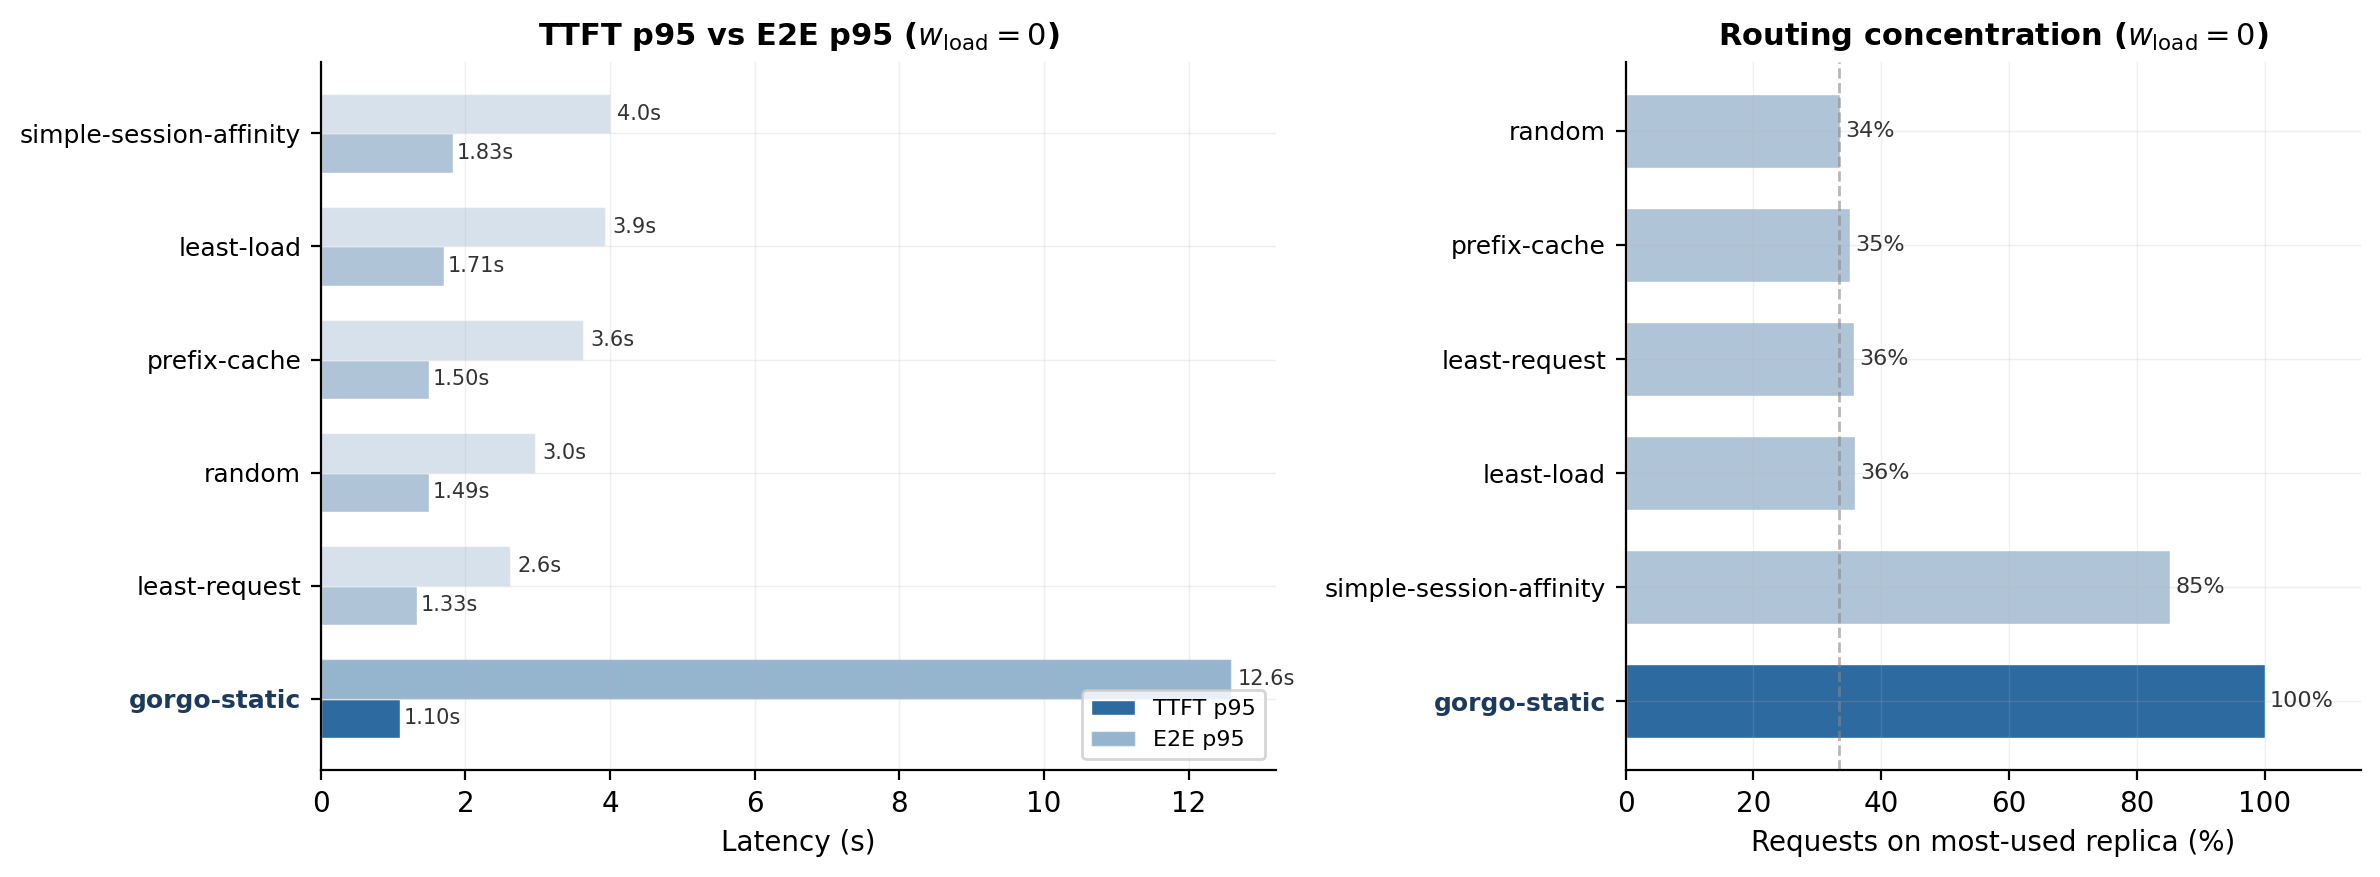
\includegraphics[width=\linewidth]{load_weight_ablation.png}
\caption{\textit{Left}: TTFT p95 (dark) vs.\ E2E p95 (light) on the midday
  diurnal trace with $w_{\mathrm{load}}{=}0$. \texttt{gorgo-static} wins
  TTFT but its E2E inflates to 12.6\,s. \textit{Right}: routing concentration.
  \texttt{gorgo-static} sends 100\% of requests to one replica.}
\label{fig:load_ablation}
\end{figure}

\end{document}